\documentclass{article}
\usepackage{tikz}
\usetikzlibrary{shapes.geometric, arrows}
%
\tikzstyle{startstop} = [rectangle, rounded corners, minimum width=3cm, minimum height=1cm,text centered, draw=black, fill=red!30]
\tikzstyle{io} = [trapezium, trapezium left angle=70, trapezium right angle=110, minimum width=3cm, minimum height=1cm, text centered, draw=black, fill=blue!30]
\tikzstyle{process} = [rectangle, minimum width=3cm, minimum height=1cm, text centered, draw=black, fill=orange!30]
\tikzstyle{decision} = [diamond, minimum width=3cm, minimum height=1cm, text centered, draw=black, fill=green!30]
\tikzstyle{arrow} = [thick,->,>=stealth]
%
\begin{document}
%
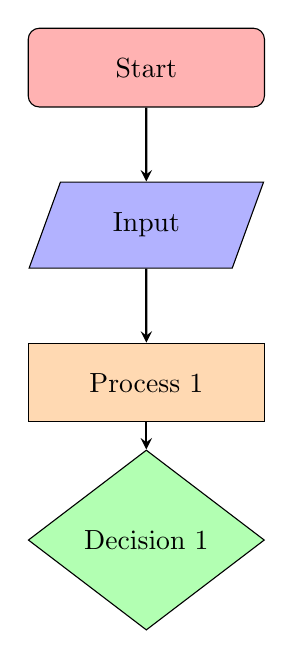
\begin{tikzpicture}[node distance=2cm]
  \node (start) [startstop] {Start};
  \node (in1) [io, below of=start] {Input};
  \node (pro1) [process, below of=in1] {Process 1};
  \node (dec1) [decision, below of=pro1] {Decision 1};
  \draw [arrow] (start) -- (in1);
  \draw [arrow] (in1) -- (pro1);
  \draw [arrow] (pro1) -- (dec1);
\end{tikzpicture}
\end{document}